\documentclass{article}
\usepackage{a4}
\usepackage{url}
\usepackage{moreverb}
% graphicx package, useful for including eps and pdf graphics
% include graphics with the command \includegraphics
\usepackage{graphicx}

\begin{document}

\newcommand{\PALMA}{{\sl PALMA}}
\newcommand{\PALMapper}{{\sl PALMapper}}
\newcommand{\GM}{{\sl GenomeMapper}}
\newcommand{\Galaxy}{{\sl Galaxy}}
\newcommand{\mGene}{{\sl mGene}}
\newcommand{\ASP}{{\sl ASP}}
\newcommand{\evaluationToolbox}{{\sl evaluationToolbox}}
\newcommand{\QP}{{\sl QPALMA}}
\newcommand{\QPA}{{\sl QPALMA alignment algorithm }}
\newcommand{\QPH}{{\sl QPALMA approximation }}
\newcommand{\QPP}{{\sl QPALMA pipeline }}
\newcommand{\qparam}[1]{{\bf #1}}



\setlength{\parindent}{0cm}


\title{PALMapper Documentation}
\author{G\'eraldine Jean}
\date{December 2010}

\maketitle
%
%
%

\section{Overview}
\label{sec:overview}
\QP{}~\cite{DeBona08} is a component of \PALMapper{}~\cite{Palmapper},
an alignment tool targeted to accurately and efficiently align both
unspliced and spliced reads produced by Next Generation sequencing
platforms such as \emph{Illumina Genome Analyzer} or
\emph{454}. \PALMapper{} is designed to deal with the relatively short
length and the possible low quality of reads by combining both the
training algorithm and the alignment component of \QP{} with the
efficient read mapping algorithm of \GM{}~\cite{GenomeMapper}. 

\QP{} relies on a machine learning strategy similar to Support Vector
Machine (SVM) and provides a scoring function to optimally combine
several pieces of information, in particular, the (a) alignment
information, (b) computational splice-site predictions, (c) read
quality values and (d) (optionally) intron lengths. This \QP{}
scoring model is then used by \PALMapper{} to guide a semi-global
alignment algorithm that allows for long gaps that correspond to
introns. For further details on \QP{} itself consult the paper
\cite{DeBona08}. For details about the learning method see
\cite{Tsochantaridis04}.

This documentation describes how to install the training component of
\QP{} and how to train it based on (a) the reference genome, (b) a 
set of RNA-seq reads,  and (c) a small set of annotated (spliced)
transcripts. 

For further information, you may contact:
\begin{center}
Gunnar R\"atsch (Gunnar.Raetsch@tuebingen.mpg.de)\\
G\'eraldine Jean (gjean@tuebingen.mpg.de)
\end{center}


\section{Installation}
\label{sec:installation}

\subsection{Dependencies}
\label{sec:dependencies}
\PALMapper{} is designed to run on \emph{Linux}/UNIX or \emph{Mac OS X} platforms and
can be downloaded at this address:\\
\url{http://ftp.tuebingen.mpg.de/pub/fml/raetsch-lab/software}.\\
This package is distributed under the GNU Public License (GPL). Read
the license before installation. The programs are distributed as C++
source. The memory requirement of \PALMapper{} depends on which kind of index is used:
\begin{itemize}
\item GenomeMapper index: it needs about seven times the genome size
  of main memory (four times for the index, about two times for
  splice-site predictions, and one time the genome size as working
  memory). In this case, \PALMapper{} requires about 21 GB of memory
  for the human genome. 
\item Bwa index: TODO
\end{itemize}
The machine’s architecture does not significantly influence the memory requirement for
these program.\\

The software package has the following dependencies on other packages:
\begin{itemize}
\item C++ compiler, for instance GNU C/C++ Compiler gcc/g++
(http://www.gnu.org). For other compilers, the compiler flags may need to be
adapted in the Makefile file.
\item Standard programs, such as \texttt{wget}, \texttt{make}, etc.
\item SAMtools for manipulating alignments in the SAM format
(http://samtools.sourceforge.net/).
\end{itemize}

\subsection{Step by step installation guide}
\label{sec:installguide}

\begin{enumerate}
\item Go to \url{http://ftp.tuebingen.mpg.de/pub/fml/raetsch-lab/software/}
    and download the package \texttt{palmapper/palmapper-0.4.tar.gz}
    to the home directory. 

\item Extract the tar-gzipped file in your home directory as follows:
\begin{verbatim}user:~$ cd
user:~$ tar zxvf palmapper-0.4.tar.gz\end{verbatim}
This command decompresses and unpacks the different files contained in
the archive to a directory named \texttt{palmapper-0.4}.

\item Compile \PALMapper{} by typing:
\begin{verbatim}user:~$ cd palmapper-0.4
user:~/palmapper-0.4$ make\end{verbatim}
Two binary files are created in the working directory: \texttt{palmapper} (the
mapping program) and \texttt{pmindex} (genome array-based index
builder). An other binary file named \texttt{bwa} is created under
\texttt{src/bwa/} and is used for building a genome bwa index.
\end{enumerate}

\section{Generating alignments with PALMapper}
\label{sec:aligning}

%%TODO: rewrite without protocol references
This section describes how to use \PALMapper{} for generating both unspliced
and spliced alignments for a set of RNA-Seq reads on the command-
line. A Galaxy version is described in Alternate Protocol
2. Using the Galaxy environment to run PALMapper is ideal if the user does not want
to worry about storage or installation. However, the current Galaxy version does not
provide enough resources to run PALMapper on big genomes such as Human; for this
case, the user should prefer the command-line version to carry out the study (see memory
requirements in Support Protocol 1).
This section shows how to run \PALMapper{} with the consideration that \QP{} has
been already trained (see TODO) and optionally splice sites have been predicted
(see TODO) for the organism of interest. Finally, the protocol describes a
test case included in the package that checks whether \PALMapper{} gives the expected
results. Results can then be used for evaluation (see TODO) and
vizualisation.

\subsection{Input files}
\label{sec:inputfile}
Aligning with \PALMapper{} needs the following files: 
\begin{itemize}
\item Genome sequence in FASTA format
\item Read data to align in Sanger FASTQ format (see section
  \ref{sec:readfile} for Sanger FASTQ format).
\item Genome annotation in GFF3 format.
\item Donor and acceptor splice-site predictions in SPF format and
corresponding binary files (optional; see section
\ref{sec:splicescoresfile} for BSPF format). There are two ways for
obtaining these files: splice site predictions can be computed for a
given genome via an appropriate tool (see
\mGene{}~\cite{Schweikertetal09,Schweikertetal09b} or
\ASP{}~\cite{Sonnenburgetal07} for example). It can be done using the
Galaxy system (\url{http://galaxy.tuebingen.mpg.de/}) and then
downloaded for local use. Alternatively, the user can directly
download precomputed splice site predictions for a growing list of
organisms at
\url{http://ftp.tuebingen.mpg.de/pub/fml/raetsch-lab/predictions/splice}. In
this case, the splice site predictions have to be used together
with the corresponding version of genome sequence. Splice-site
predictions and the corresponding version of the genome can be easily
downloaded by running the command: 
\begin{verbatim}
user:~/palmapper-0.4/splice_predictions$ make <organism>
\end{verbatim}
where \texttt{<organism>} is the name of the organism of interest.\\
The user may also disable the use of splice site predictions by using
\texttt{-no-ss-pred} parameter in the way explained in step 3 below.
\item \QP{} parameter file (see
  Figure~\ref{fig:qp_parameter_file}). This file is obtained by
  training \QP{} (for more information, consult the comprehensive tutorial
  paper about \PALMapper{}~\cite{Palmapper}). Pretrained \QP{}
  parameter files for use with \PALMapper{} are located 
in: \texttt{~/palmapper-0.4/qpalma\_parameters}. Be sure to read the
README file in the same directory for more information.
\end{itemize}

\begin{figure}[h!]
\begin{center}
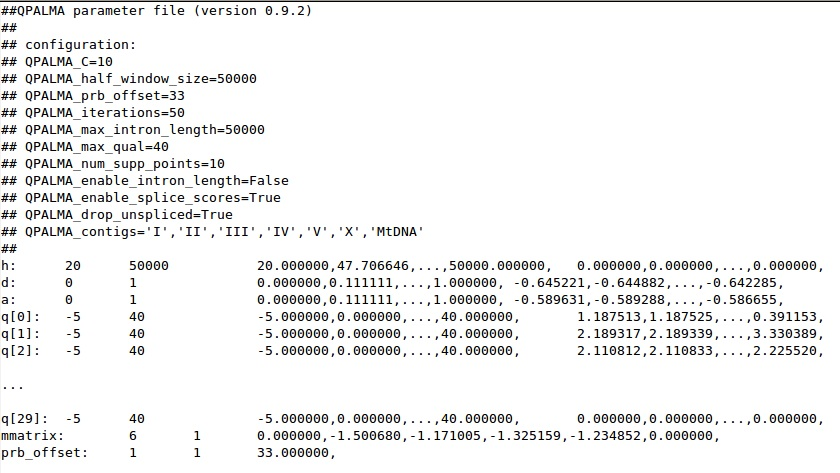
\includegraphics[width=\textwidth]{QPALMAFile.jpg}
\end{center}
\caption{Example of a \QP{} parameter file generated during the training
  phase of \QP{}. The first lines starting with $\#\#$ characters
  describe the parameters used for generating this file. The following
  lines represent the piece-wise linear functions for intron length (h),
  donor splice sites (d), acceptor splice sites (a) and edit operations
  for match/mismatch/gap on read (q). Each piece-wise linear function is
  defined by the range of possible x-values (length for h, splice site
  predictions for d and a, quality for q) which is followed by the
  values for all support points (first, x-values separated by commas
  then, after a space, y-values separated by commas
  too). \texttt{mmatrix} defines fixed scores for a gap on DNA according
  to possible aligned base in read. Finally, \texttt{prb\_offset} is the
  quality offset for determining the quality value from the ASCII
  quality character.}
\label{fig:qp_parameter_file}
\end{figure}

\subsection{Aligning with PALMapper on the command-line}
\label{sec:aligningcl}

\begin{enumerate}
\item Create an index of the reference genome:\\
\PALMapper{} offers the possibility to use two different kinds of
index for the reference genome: array-based and bwa. The first one
uses more space but provides a better runtime. We advise the user to
use array-based index for genomes of small size (\emph{C. Elegans} for
instance) and the bwa index for large genomes as \emph{Human}.
\begin{itemize}
\item[a] Create an array-based index:
\begin{verbatim}
user:~$ cd palmapper-0.4/
user:~/palmapper-0.4$ ./pmindex -i <genome_file> -s <index_size> -v
\end{verbatim}
where \texttt{<index\_size>} is the seed length used during indexing
(e.g., 13). This creates 4 files the prefix of which is
\texttt{<genome\_file>}:
\begin{itemize}
\item \texttt{<genome\_file>.cid}: chromosome index file
\item \texttt{<genome\_file>.mta}: meta index file
\item \texttt{<genome\_file>.mfd}: forward index file
\item \texttt{<genome\_file>.mrc}: reverse index file
\end{itemize}

\item [b] Create a bwa index:
\begin{verbatim}
user:~$ cd palmapper-0.4/src/bwa
user:~/palmapper-0.4/src/bwa$ ./bwa index <genome_file>
\end{verbatim}
This creates 4 files the prefix of which is \texttt{<genome\_file>}:
\begin{itemize}
\item \texttt{<genome\_file>.bwt}: forward index file
\item \texttt{<genome\_file>.rbwt}: reverse index file
\item \texttt{<genome\_file>.sa}: suffix array for forward index
\item \texttt{<genome\_file>.rsa}: reversed suffix array for reverse
  index file
\end{itemize}
\end{itemize}

\item Use the command below to run \PALMapper{} within the working directory. The
command provided here is a generic one for computing both unspliced and spliced
alignments (spliced via \texttt{-S} option), and the user should
revise the options described in TODO and TODO for best results.
\begin{verbatim}
user:~/palmapper-0.4$ ./palmapper -i <genome_file> -q <read_file> \
[OPTIONS_PALMAPPER] -S -qpalma <qpalma_param_file> \
-acc <acc_pred_file> -don <don_acc_file> -o <out_mapped_file> \
-u <out_unmapped_file> [OPTIONS_QPALMA]
\end{verbatim}

where:
\begin{itemize}
\item \texttt{<genome\_file>} is the path to the genome sequence file.
\item \texttt{<read\_file>} is the path to the genome read data file.
\item \texttt{<qpalma\_param \_file>} is the path to the \QP{} parameter file.
\item \texttt{<acc\_pred\_file>}, \texttt{<don\_pred\_file>} are the paths to acceptor and
donor splice-site prediction files. Replace both of these parameters
by \texttt{no-ss-pred} option if you want to disable the use of splice
site predictions during the alignment process. In this case, use a
\QP{} parameter file obtained by training QP{} without using splice
site predictions.
\item \texttt{<out\_mapped\_file>}, \texttt{<out\_unmapped\_file>}
are the paths to the alignment output and the unmapped reads files.
See Tables TODO and TODO for details about \texttt{[OPTIONS\_PALMAPPER]} and
\texttt{[OPTIONS\_QPALMA]}, respectively.
\end{itemize}
By default, the array-based index is used to generate alignments. To
switch to bwt-based index, the user should add the option \texttt{-bwa} in
the command-line.
\item Two output files are generated and are located according to the specified paths
\texttt{<out\_mapped\_file>}, and \texttt{<out\_unmapped\_file>}:
\begin{itemize}
\item An alignment file, which stores all alignments of reads for which an alignment
satisfying the specified criteria has been found.
\item An unmapped read file, which stores all reads for which no alignment has been
found. The \texttt{-u} option is optional.
\end{itemize}
By default, the alignment file is encoded in a SAM format but the user can alternatively
choose between BED, an extended BED format (BEDx), SHORE, and SAM formats using
the option \texttt{-f}. The unmapped reads are written in FASTQ
format. See sections~\ref{sec:readfile} and \ref{sec:samfile} for
specifications of FASTQ and SAM formats, respectively.

\item \emph{Optional}: Convert alignment files in SAM format into
  wiggle VariableStep format by running the following commands:
\begin{verbatim}
user:~/palmapper-0.4$ cd tools/
user:~/palmapper-0.4/tools/$ python sam2wig.py --input=<alignment_file> \
--ref-file=<genome_file> --output=<wiggle_file> --expName=<exp_name> \
\end{verbatim}

where \texttt{<alignment\_file>} is the path to alignment file
obtained in step 3, \texttt{<genome\_file>} is the path to the
sequence file of reference genome, \texttt{<wiggle\_file>} is the path
to output wiggle VariableStep file, and \texttt{<exp\_name>} is the
name the user wants to give to his experiment (e.g., Experiment
SRX001872). Alternatively, one may use the
\texttt{-report-coverage-wig} option to generate the coverage wiggle
file directly. Wiggle VariableStep files are necessary if you want to
visualize the resulting alignments using a genome browser (GBrowse for
instance) or Galaxy Trackster.  
\end{enumerate}


\subsection{Aligning with PALMapper on an example}
\label{sec:example}

\begin{enumerate}
\item Open a new shell window and go to \texttt{testcase} directory by
  typing: 
\begin{verbatim}
user:~$ cd palmapper-0.4/testcase/
\end{verbatim}
The user can easily test \PALMapper{} on an example from
\emph{C. elegans} that is ready to run in the testcase directory of
\PALMapper{} package.
\item Run test case by typing:
\begin{verbatim}
user:~/palmapper-0.4/testcase$ make test
\end{verbatim}
This command first downloads splice-site predictions and the
\emph{C. elegans WS209} reference sequence. Then, it runs \PALMapper{}
using the following detailed command:
\begin{verbatim}
../palmapper -i data/c_elegans.WS209.dna.fa -q data/split_1m.000 \
-acc data/C_elegans_SpliceSitePred_WS209/acc_pred.bspf/contig_%i%c \
-don data/C_elegans_SpliceSitePred_WS209/don_pred.bspf/contig_%i%c \
-o data/split 1m.000.sam -u data/split_1m.000.unmapped \
-S -f sam -report-coverage-wig data/split_1m.000.wiggle -qpalma \
data/parameters.qpalma \
-M 4 -G 1 -E 4 -l 20 -L 35 -K 12 -C 55 -z 1 \
-seed-hit-cancel-threshold 1000
\end{verbatim}
The output files in SAM format (see section~\ref{sec:samfile}) are
stored in \texttt{./palmapper-0.4/testcase/data/}. Finally, the
program checks if \PALMapper{} has correctly run by comparing obtained
results with precomputed results on the same data set. The user should
see the following information confirming that produced results are
those expected appear in the shell window: 

\begin{verbatim}
split 1m.000.sam: OK
split 1m.000.unmapped: OK
split 1m.000.wiggle: OK
\end{verbatim}

This command uses array-based index files to run the testcase. To do
the same testcase using bwt-based index, type \texttt{make bwamap}
instead of \texttt{make test}. Results should be the same.
\end{enumerate}

\section{Aligning with PALMapper using Galaxy tools}
\label{sec:aligninggal}
\PALMapper{} can also be used via a Web service
(\url{http://galaxy.fml.mpg.de/}), which is a customized version of
the Galaxy frameworks~\cite{Galaxy1,Galaxy2,Galaxy3}. There are no
difference between these two ways of using \PALMapper{} except that using
galaxy saves the user from installing the software. Moreover, it is
preferable to align with \PALMapper{} via galaxy if the rest of the study is
carried out with galaxy as well. For further details about how to
align with \PALMapper{} using Galaxy tools, please read \PALMapper{}
tutorial \cite{Palmapper}.


% \label{sec:training}
% This section describes how to train the \QP{} component of \PALMapper{}
% based on the reference genome, a set of RNA-seq reads and a small set
% of annotated (spliced) transcripts. During this process an  
% error model is estimated from a preliminary alignment of the reads to
% the reference genome and a set of artificial reads is created from the
% annotated transcripts and the error model. Both steps are necessary to
% generate a set of realistic artificial reads with known alignment in
% order to train \QP{}. The training and later the alignment benefit
% from computational splice sites predictions for the reference
% genome. The result of the training step is a \QP{} parameter file
% adapted to the specifics of the reads of an RNA-seq experiment, which
% is required for the alignment protocol.\\ 
% The \QP{} and \PALMapper{} releases also contain pre-trained \QP{}
% parameter files, which can be used alternatively. It should be noted,
% however, that the \QP{} parameters optimally trade-off the amount
% errors in the reads and the information from splice site predictions
% for one combination of RNA-seq experiment, splice site predictions and
% genome. Using sharing parameter sets among experiments or genome can
% lead to a suboptimal alignment performance with \PALMapper{}. 


\section{File Formats / Specifications}
\label{sec:formats}
This section introduces all formats and conventions to be used when
aligning with \PALMapper{}.

\subsection{The read file}
\label{sec:readfile}

The read file is encoded in Sanger FASTQ format. A FASTQ file normally
uses four lines per sequence. The first line begins with a '@'
character and is followed by the read identifier and an optional
description. The second line is the nucleotide sequence of the
read. The third line begins with a '+' character and is optionally
followed by the same identifier (and any description) again than in
line 1. The last line encodes the quality values for the sequence in
line 2, and must contain the same number of symbols as letters in the
sequence. Sanger format encodes a quality score from 0 to 93 using ASCII
33 to 126. For a more detailed description of the FASTQ format consult:
\url{http://en.wikipedia.org/wiki/FASTQ_format}. Figure~\ref{fig:fastq}
is an example of a Sanger FASTQ file.

\begin{figure}[h!]
\begin{center}
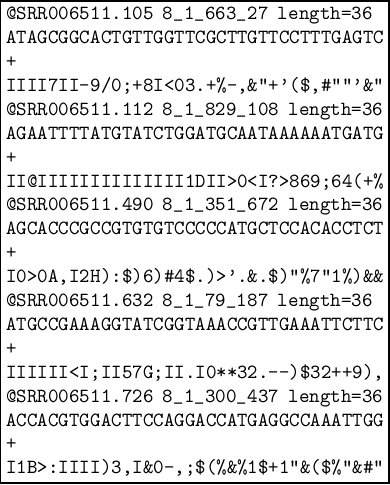
\includegraphics[width=0.5\textwidth]{ReadFile.jpg}
\end{center}
\caption{Example of a Sanger FASTQ file for input read data.}
\label{fig:fastq}
\end{figure}

\subsection{Splice Scores}
\label{sec:splicescoresfile}

As mentioned before, the splice site scores can be generated using an
appropriate tool such that
mGene~\cite{Schweikertetal09,Schweikertetal09b} or
ASP~\cite{Sonnenburgetal07}. If you would like to use your own splice
site 
predictions you can create files according to the Binary Signal
Prediction Format (BSPF) described below: 

For each canonical acceptor ($AG$) and donor site ($GT$/$GC$)
\QP{} expects a score. The data is organized in files for each signal
(acc/don) for each strand (+/-).  The information on positions of
canonical splice sites and the corresponding scores lies in separate
files. Every chromosome or contig leads then to $8$ files (acc/don, +/-
and pos/score). The position and score files are raw binary files
containing the ordered positions and the scores. The positions are
stored as unsigned values and the scores as floats. Note that you have
to be careful when working in an inhomogeneous cluster environment
(endianness, data type size). The positions are 1-based and the
assignment of positions and their scores is as follows: The acceptor
score positions are the positions right after the $AG$ and the donor
score positions are the positions right on the $G$ of the $GT$ or
$GC$. For example:
\begin{center}
\begin{tabular}{ccccccccccc}
... & 3 & 4 & 5 & 6 & 7 & 8 & 9 & 10 & 11 & ... \\ 
... & w & g & t & x & y & z & a & g  & v  & ... \\
... &   & 0.2&  &   &   &   &   &    & 0.3 & ... 
\end{tabular}
\end{center}

\subsection{Alignment file}
\label{sec:samfile}


\section{General settings}
\label{sec:settings}

\subsection{GenomeMapper settings}
\label{sec:settingsgm}

\subsection{QPALMA settings}
\label{sec:settingsqp}


\section{Internet Resources}
\url{http://www.fml.mpg.de/raetsch/suppl/palmapper}\\
\emph{\PALMapper{} project web-page.}\\
\url{http://www.fml.mpg.de/raetsch/suppl/palmapper/tutorial}\\
\emph{\PALMapper{} tutorial web-page.}\\
\url{http://www.fml.mpg.de/raetsch/suppl/qpalma}\\
\emph{\QP{} project web-page.}\\
\url{http://www.fml.mpg.de/raetsch/suppl/mgene}\\
\emph{\mGene{} project web-page.}\\
\url{http://www.fml.mpg.de/raetsch/suppl/splice}\\
\emph{\ASP{} project web-page.}\\
\url{http://ftp.tuebingen.mpg.de/pub/fml/raetsch-lab/software/}\\
\emph{http server for downloading \QP{}.}\\
\url{http://galaxy.fml.mpg.de/}\\
\emph{\Galaxy{} server.}\\

%
% Bibliography
% 

\begin{thebibliography}{1}

\bibitem[1]{DeBona08} 
  \newblock F.~De~Bona, S.~Ossowski, K.~Schneeberger, and G.~R{\"a}tsch.
  \newblock Optimal Spliced Alignment of Short Sequence Reads.
  \newblock {\em Bioinformatics}, 24(16):i174-i180, 2008.

\bibitem[2]{Palmapper} 
  \newblock G.~Jean, A.~Kahles, V.T.~Sreedharan, F.~De~Bona, and G.~R\"atsch.
  \newblock RNA-Seq Read Alignments with PALMapper.
  \newblock {\em Curr. Protoc. Bioinformatics}, 32:11.6.1-11.6.38, 2010.

\bibitem[3]{GenomeMapper}
  \newblock K.~Schneeberger, J.~Hagmann, S.~Ossowski, N.~Warthmann,
  S.~Gesing, O.~Kohlbacher, and D.~Weigel. 
  \newblock Simultaneous alignment of short reads against multiple genomes.
  \newblock {\em Genome Biology}, 10(9):R98, 2009.

\bibitem[4]{Tsochantaridis04} 
  \newblock I.~Tsochantaridis, T.~Hofmann, T.~Joachims and Y.~Altun.
  \newblock Support Vector Machine Learning for Interdependent and Structured Output Spaces.
  \newblock {\em Proceedings of the 16th International Conference on Machine Learning}, 2004.

\bibitem[5]{Schweikertetal09}
  \newblock G.~Schweikert, G.~Zeller, A.~Zien, J.~Behr, C.-S.~Ong, P.~Philips,
  A.~Bohlen, S.~Sonnenburg, and G.~R\"atsch.
  \newblock {mGene}: {A} Novel Discriminative Gene Finding System.
  \newblock {\em Genome Research}, 19:2133-2143, 2009.

\bibitem[6]{Schweikertetal09b}
  \newblock G.~Schweikert, J.~Behr, A.~Zien, G.~Zeller, S.~Sonnenburg, and G.~R\"atsch.
  \newblock mGene.web: a web service for accurate computational gene
  finding. 
  \newblock {\em Nucleic Acids Research}, 37(Suppl. 2):W312–W316, 2009. 

\bibitem[7]{Sonnenburgetal07}
  \newblock S.~Sonnenburg, G.~Schweikert, P.~Philips, J.~Behr, and
  G.~R{\"a}tsch. 
  \newblock Accurate splice site prediction using support vector machines.
  \newblock {\em BMC Bioinformatics}, 8(Suppl 10):S7, 2007.

\bibitem[8]{Galaxy1}
  \newblock D.~Blankenberg, J.~Taylor, I.~Schenck, J.~ He, Y.~Zhang,
  M.~Ghent, N.~Veeraraghavan, I.~Albert, W.~Miller, K.~Makova, R.~Hardison, and A.~Nekrutenko.
  \newblock A framework for collaborative analysis of ENCODE data: making large­scale analyses biologist-friendly.
  \newblock {\em  Genome Research}, 17(6):960–964, 2007. 

\bibitem[9]{Galaxy2}
  \newblock J.~Taylor, I.~Schenck, D.~Blankenberg, and A.~Nekrutenko.
  \newblock Using galaxy to perform large-scale interactive data
  analyses. 
  \newblock {\em Curr. Protoc. Bioinformatics}, 19:10.5.1-10.5.25, 2007. 

\bibitem[10]{Galaxy3}
  \newblock D.~Blankenberg, G.~Von~Kuster, N.~Coraor, G.~Ananda,
  R.~Lazarus, M.~Mangan, A.~Nekrutenko, J.~Taylor.
  \newblock Galaxy: A Web­Based Genome Analysis Tool for Experimentalists.
  \newblock {\em Curr. Protoc. Molecular Biology}, 89:19.10.1-19.10.21, 2010.


  



\end{thebibliography}
%
%
%
\end{document}
